\chapter{Double Beta Decay}
\label{chap:Beta Decay}

While a lepton-violating process such as that in \autoref{fig:0nuBB} would an incredible result to discover in the laboratory, it's not quite so simple as to obtain a ``soup" of down quarks and wait for them to decay into up quarks and electrons or to look at the time-reversed process and use electron beams to produce up and down quarks!
The way that an interaction such as the one shown above in \autoref{fig:0nuBB} could feasibly be discovered in a laboratory setting is through decays of nuclei, namely through neutrinoless double-beta decay, \zeronubb. 
\section{Beta Decay}
\label{sec:Beta Decay}
\zeronubb~decay is an extension on a well-known and well-understood process called beta decay. In beta decay, a decay that occurs in many nuclei, the number of protons, Z, in the nucleus changes while the number of total nucleons, A, is constant.
Beta decay occurs in two main processes and can be described in the following nuclear decays
\begin{align}
    (Z, A) & \rightarrow (Z+1, A)+\textrm{e}+\Bar{\nu}_e \label{eq:neutrondecay} \\
    (Z, A) & \rightarrow (Z-1, A)+\Bar{\textrm{e}}+\nu_e. \label{eq:protondecay}
\end{align}
\begin{figure}[tbph]
    \centering
    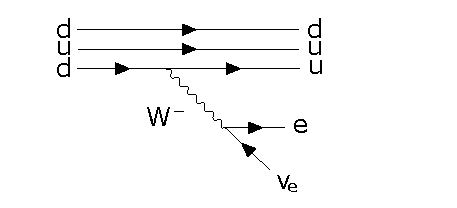
\includegraphics[width=0.8\linewidth]{Figures/NeutronBetaDecay.pdf}
    \caption[Beta Decay Feynman diagram for a neutron converting to a proton.]
    {The Feynman diagram for beta decay for a neutron to convert to a proton inside a nucleus by emitting an electron and and anti-neutrino.}
    \label{fig:NeutronBetaDecay}
\end{figure}
The process in \autoref{eq:neutrondecay} is shown in \autoref{fig:NeutronBetaDecay}, and the accompanying process, \autoref{eq:protondecay}, while kinematically forbidden in free protons because protons have less mass than neutrons, is able to occur in nuclei where the change in binding energies of the resultant nucleus is able to compensate for the mass difference between protons and neutrons.
When discussing these decays, an important value of interest is known as the Q-value of the decay which is the available energy released during the decay of one nucleus to another, namely (Z,A) $\rightarrow$ (Z$\pm1$, A).
This energy sets the maximum energy that can be carried off by the resultant particles and serves as the endpoint of the beta decay spectrum. 
\subsection{History of Beta Decay}
Historically, the discovery and physics advancements from double-beta decay has shed some light on new physics.
In particular, when the energy spectrum of beta decays was first discovered, it took the physics community by surprise that the spectrum was continuous and not peaked at a single value as, e.g., an alpha decay would be \cite{o.vonbayero.hahnl.meitner}.
This seemed to suggest one of two things. Either energy was not conserved in the interaction, or there was a seemingly massless undetected particle that was escaping the interaction and taking away energy.
To resolve this issue, Wolfgang Pauli speculated in a famous letter in 1930 to ``dear radioactive ladies and gentlemen" about the existence of the neutrino particle to account for the missing energy \cite{pauli_1930}.
At the time, the physics community was quite skeptical of such a theory, as it posited a particle that was seemingly impossible to detect in order to conserve energy, and Enrico Fermi was even rejected on these grounds from publishing his theory on beta decay in the journal Nature, publishing instead in a lesser-known journal \cite{fermi_1934}.
Despite the misgivings of the community, neutrinos were in fact not impossible to detect and were first discovered in the Cowan-Reines experiment only 20 years later in 1954 \cite{PhysRev.92.830}.
Using beta capture, a similar process to beta decay, this experiment observed antineutrinos interacting with ``free" protons in hydrogen atoms in a water tank. 
In this way, beta decay has been used to observe new physics and has been both an active and fruitful area of research since it was first observed.
Even recently, observations of neutrinos have resulted in the discovery of neutrino oscillations, discussed in \autoref{ssec:NeutrinoMassesandOscillation}, which was the first confirmation of physics beyond the Standard Model.
\section{Double-Beta Decay}
\label{sec:Double Beta Decay}
Since beta decay is an allowed process, a decay in which two decays happen simultaneously, double-beta decay, described in \autoref{eq:doubleneutrondecay} and \autoref{eq:doubleprotondecay} below, should also be allowed.
\begin{align}
    (Z, A) & \rightarrow (Z+2, A)+2\textrm{e}+2\Bar{\nu}_e \label{eq:doubleneutrondecay} \\
    (Z, A) & \rightarrow (Z-2, A)+2\Bar{\textrm{e}}+2\nu_e \label{eq:doubleprotondecay} 
\end{align}
However, for most nuclei, this second-order weak process is dwarfed by the significantly higher rates of single-beta decay.
Although the rate of beta decay depends greatly on the isotope, even some of the longest half-lives, such as that of $^{40}$K with a half-life of $1.251\times10^{9}~\textrm{yr}$, are many orders of magnitude faster than typical half-lives for double-beta decay, $\mathcal{O}(10^{20})~\textrm{yr}$.
This 11 orders of magnitude longer rate makes measuring double-beta decay virtually impossible as the single-beta decay rate presents an insurmountable background.
However, the exception to this occurs in some even-even nuclei wherein single beta decay is energetically forbidden, but double beta decay is allowed, shown in \autoref{fig:parabola_even}.
Of the 35 naturally-occurring isotopes where double beta decay is possible, 12 of them have been measured in the laboratory, and 9 of these are shown in \autoref{tab:2nuHalfLife}.
As the longest measured half-life of alpha decay is from $^{209}\textrm{Bi}$ with a half-life of $1.9 \times 10^{19}~\textrm{years}$ \cite{Marcillac:2003Bi-209detection}, double-beta decay half lives are the rarest nuclear decays that have been measured.
\begin{figure}[htbp]
%\captionsetup[subfigure]{justification=centering}
\centering
\begin{subfigure}[t]{0.40\textwidth}
\centering
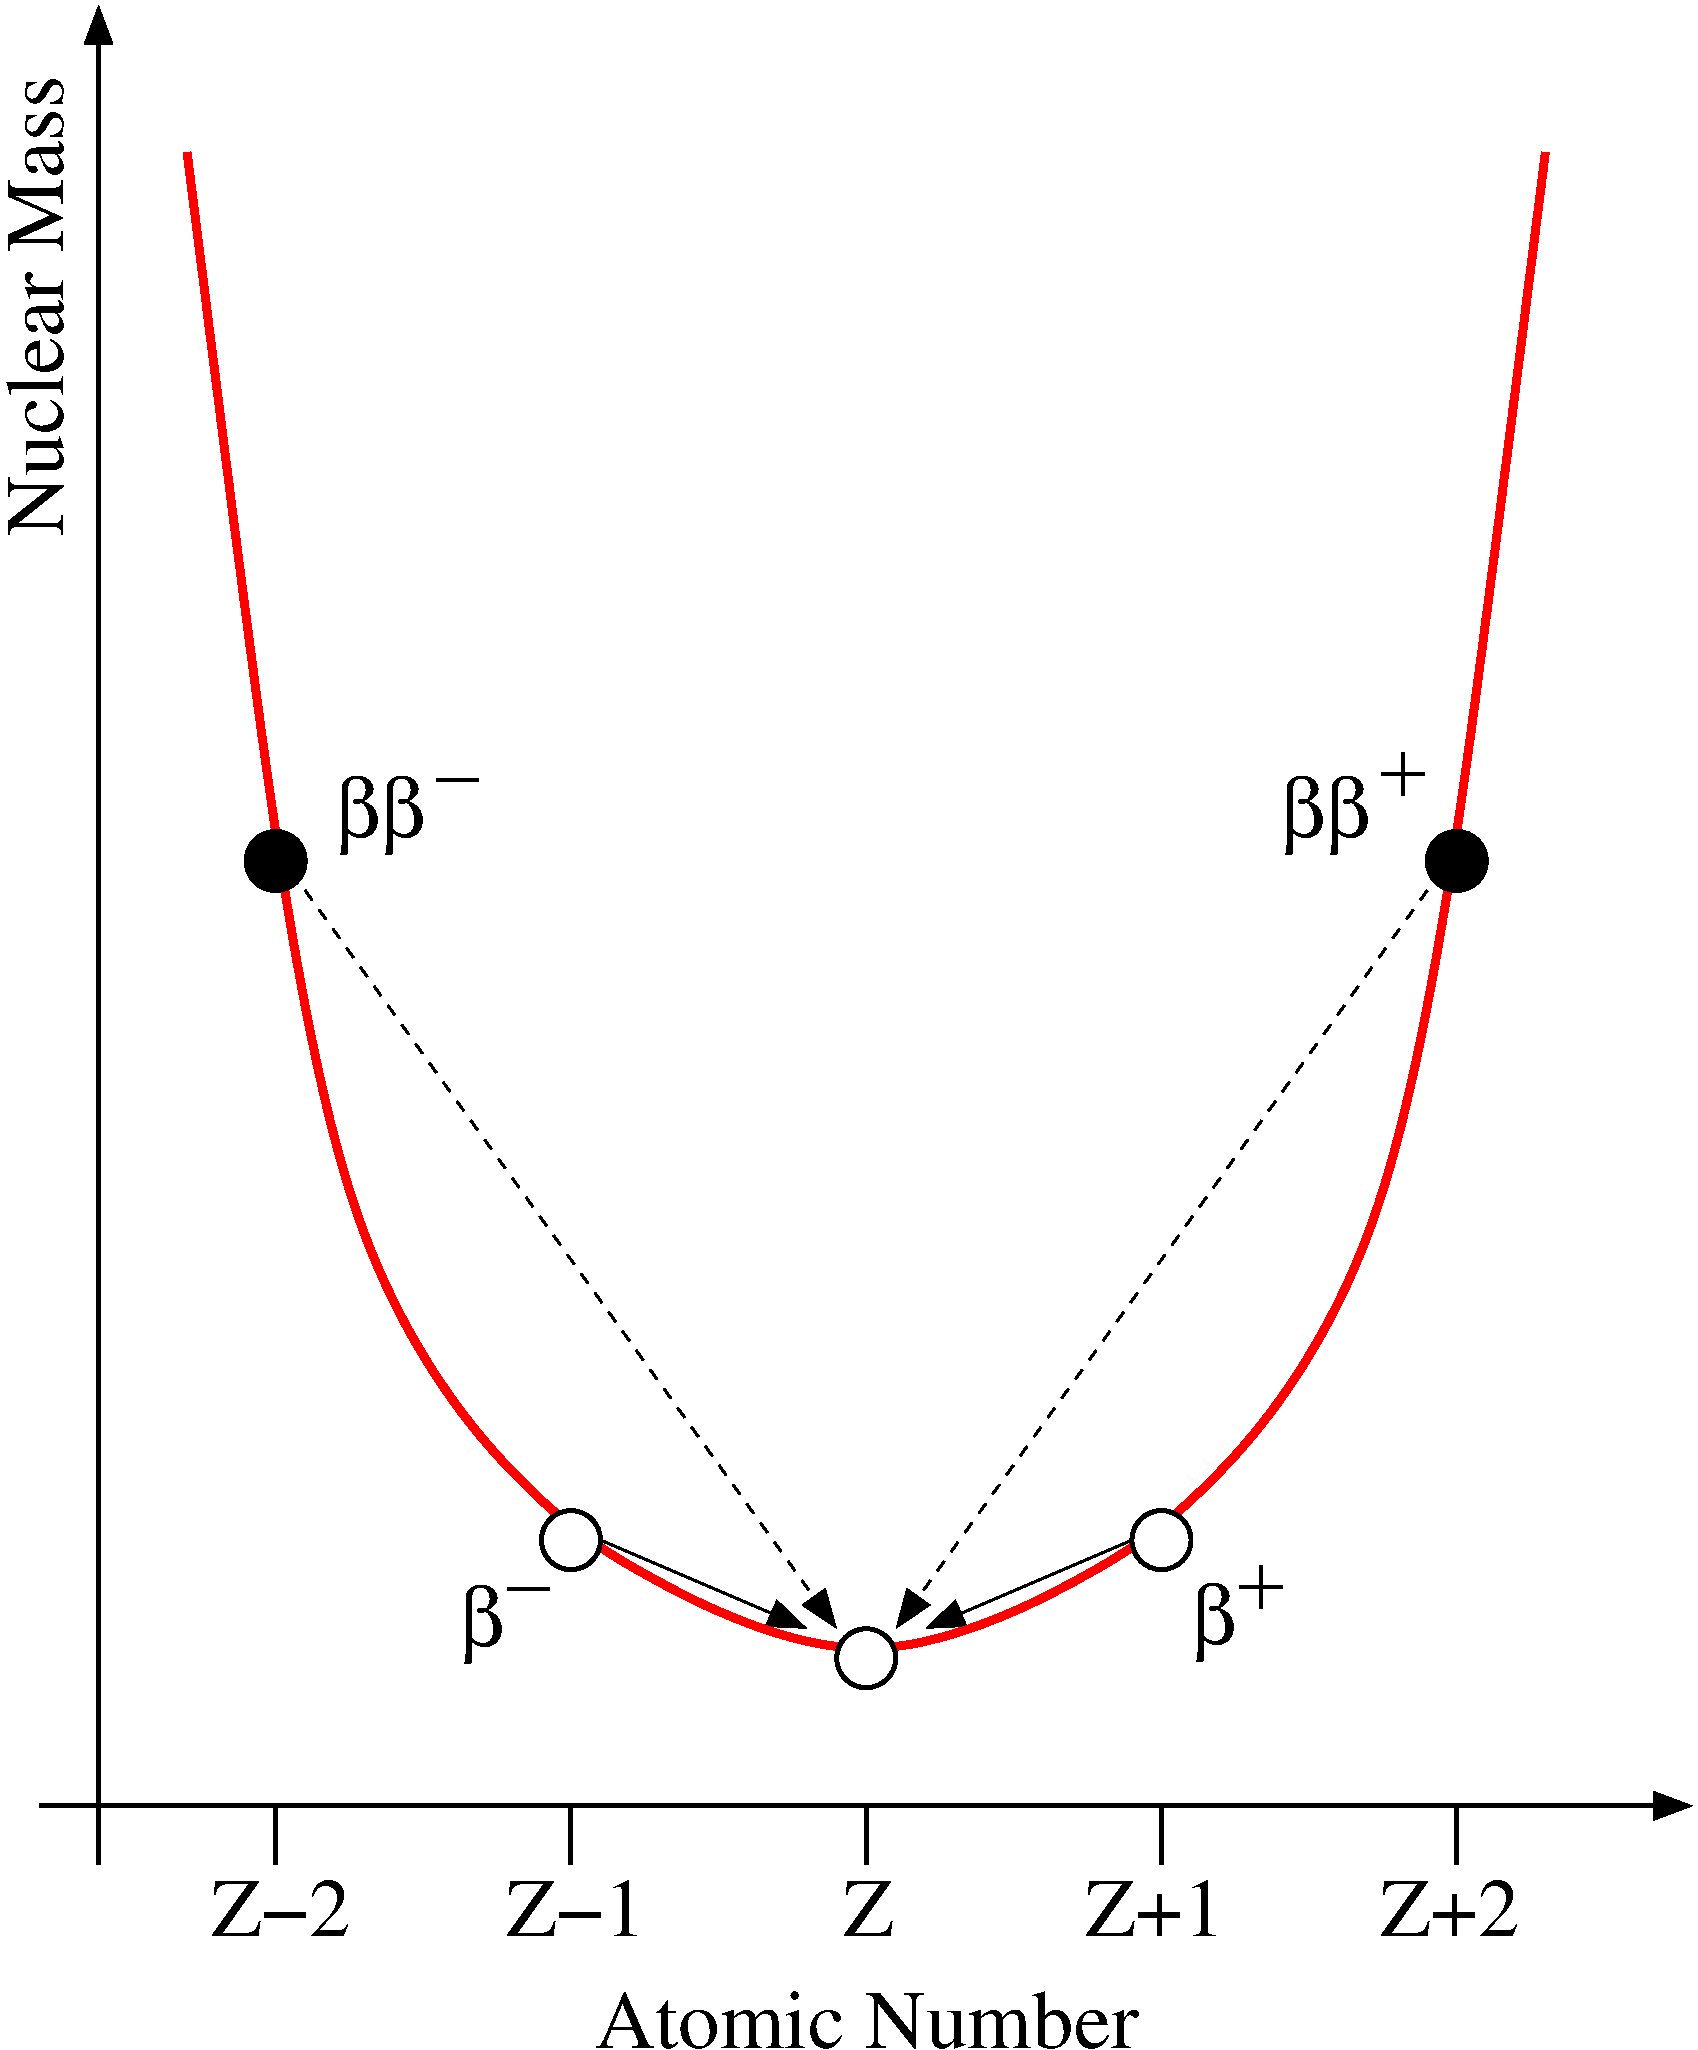
\includegraphics[width=0.9\textwidth]{Figures/parabola_odd_edited.pdf}
\caption{}
\label{fig:parabola_odd}
\end{subfigure}
\qquad
\begin{subfigure}[t]{0.40\textwidth}
\centering
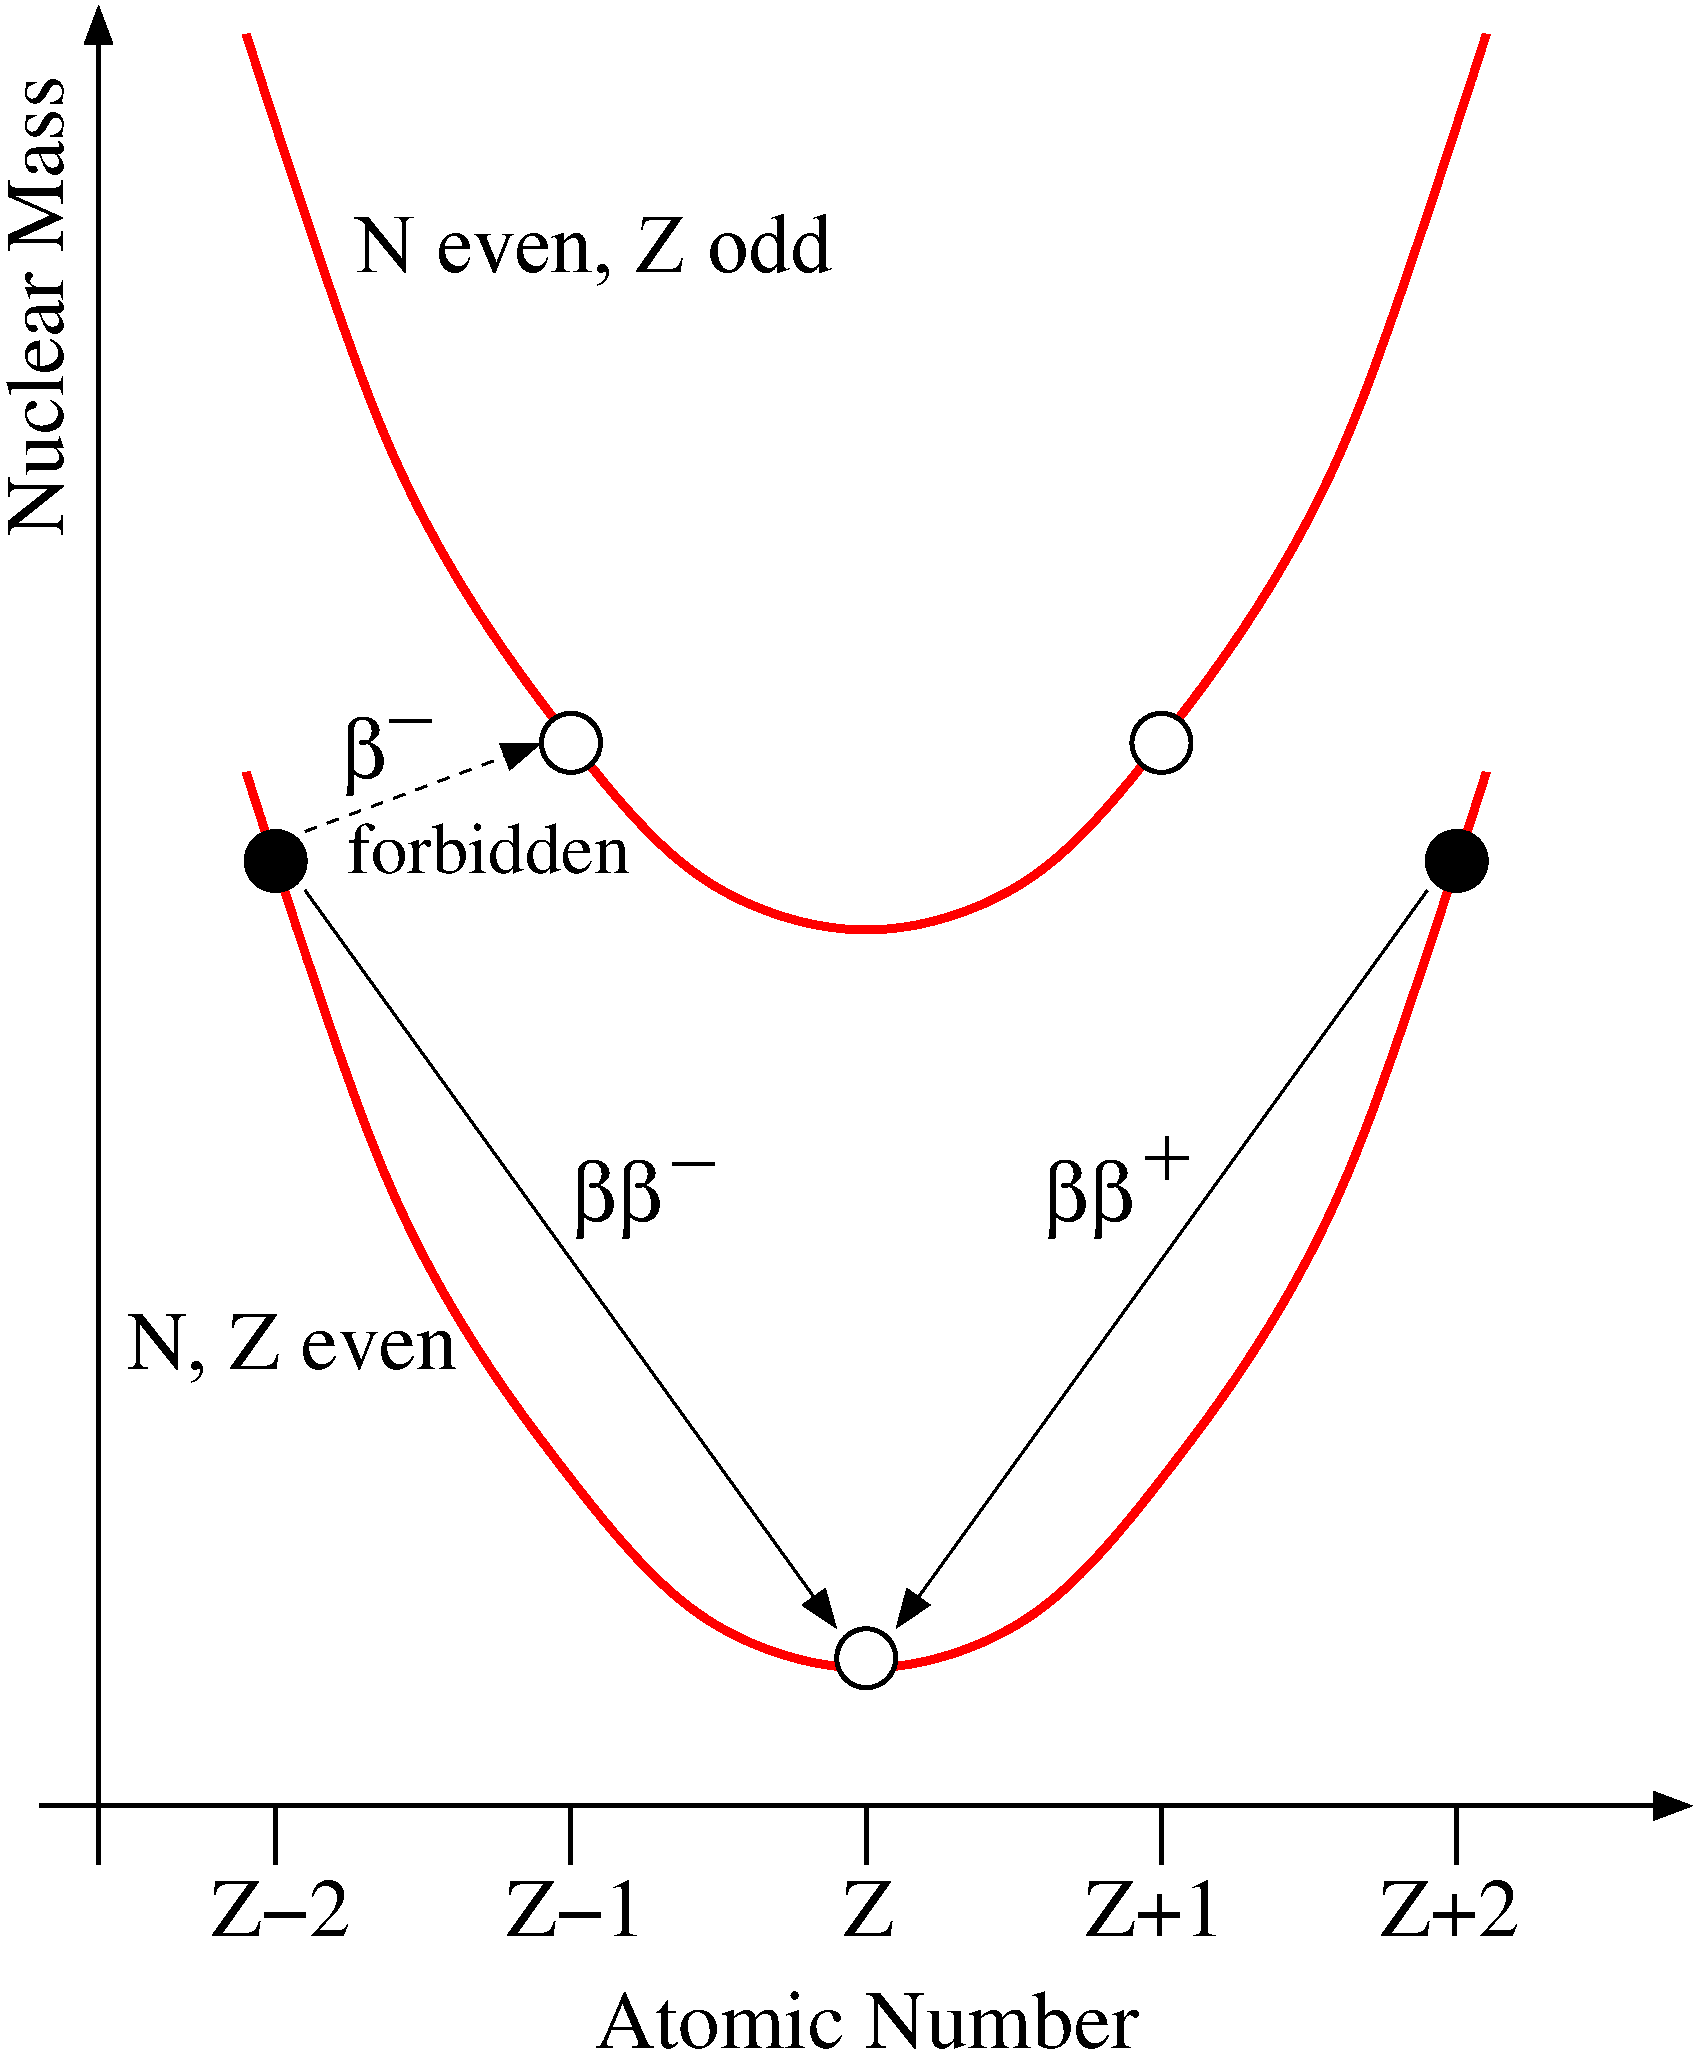
\includegraphics[width=0.9\textwidth]{Figures/parabola_even_edited.pdf}
\caption{}
\label{fig:parabola_even}
\end{subfigure}
\caption[Two sets of double-beta decay candidate nuclei.
(a) an odd mass nucleus allows for both single- and double-beta decay.
(b) an even-even nucleus allows only double-beta decay as single-beta decay is kinematically forbidden.]
{Two sets of double-beta decay candidate nuclei.
(a) an odd mass nucleus allows for both single- and double-beta decay.
(b) an even-even nucleus allows only double-beta decay as single-beta decay is kinematically forbidden.}
\label{fig:parabola_evenodd}
\end{figure}
\begin{table}[H]
\centering
\begin{tabular}{ccc}
\hline \hline
Isotope & Half-life, $10^{21}$ years & Experiment \\ \hline 
$^{48}\textrm{Ca}$ & $0.044^{+0.005}_{-0.004} \pm 0.004$\cite{Bongrand:2011ei} & Nemo-3 \\
$^{76}\textrm{Ge}$ & $1.926^{+0.025}_{-0.022} \pm 0.092$\cite{Agostini:2015nwa} & GERDA  \\
$^{82}\textrm{Se}$ & $0.096 \pm 0.003 \pm 0.010$\cite{Bongrand:2011ei} & NEMO-3 \\ 
$^{96}\textrm{Zr}$ & $0.0235 \pm 0.0014 \pm 0.0016$\cite{Bongrand:2011ei} & NEMO-3 \\ 
$^{100}\textrm{Mo}$ & $0.00711 \pm 0.00002 \pm 0.00054$\cite{Bongrand:2011ei} & NEMO-3 \\ 
$^{116}\textrm{Cd}$ & $0.028 \pm 0.001 \pm 0.003$\cite{Bongrand:2011ei} & NEMO-3 \\ 
%^{128}\textrm{Te}$ & $7200 \pm 400$ & Geochemical \\
$^{130}\textrm{Te}$ & $0.82 \pm 0.02\pm 0.06$\cite{Alduino:2016vtd} & CUORE-0 \\
$^{136}\textrm{Xe}$ & $2.165 \pm 0.016 \pm 0.059$\cite{Albert:2013gpz} & EXO-200 \\
$^{150}\textrm{Nd}$ & $0.00911^{+0.00025}_{-0.00022}\pm 0.00063$\cite{Bongrand:2011ei} & NEMO-3 \\
%$^{238}\textrm{U}$ & $2.0 \pm 0.6$ & Radiochemical \\
\hline \hline
\end{tabular} 
\caption[List of known two-neutrino beta decay half lives.]
{List of the known double-beta decay half lives along with the experiment which has the most precise measurement to date.
The order of the errors on the half-life are statistical followed by systematic.}
\label{tab:2nuHalfLife}
\end{table}
\section{Neutrinoless Double-Beta Decay}
\label{sec:Neutrinoless Double Beta Decay}
Of most interest to this thesis is a variation on the \twonubb~decay mentioned above where the neutrinos are exchanged during the decay and do not emerge as final state particles.
This corresponds to the decay shown in \autoref{fig:0nuBB} and in \autoref{eq:doubleneutrondecay_neutrinoless} and \autoref{eq:doubleprotondecay_neutrinoless} below:
\begin{align}
    (Z, A) & \rightarrow (Z+2, A)+2\textrm{e} \label{eq:doubleneutrondecay_neutrinoless} \\
    (Z, A) & \rightarrow (Z-2, A)+2\Bar{\textrm{e}}. \label{eq:doubleprotondecay_neutrinoless} 
\end{align}
In this decay, only possible if the neutrino has a Majorana mass, all of the available energy released in the decay is carried away by the electrons.
Therefore, a detector which can measure the electron energy would always reconstruct the decay energy to be precisely at the Q-value of the decay, in contrast to the energy spectrum from \twonubb~decay which is a continuum up to the Q-value due to the undetected neutrinos carrying energy away from the detectors.
\begin{figure}
    \centering
    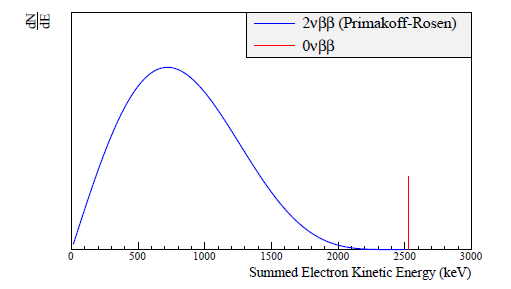
\includegraphics[width=0.6\linewidth]{Figures/2nuBBSpectrum.png}
    \caption[The energy spectrum for \twonubb~decay of $^{130}$Te along with the spectrum for \zeronubb.]
    {The energy spectrum for \twonubb~decay of $^{130}$Te along with the spectrum for \zeronubb.
    The spectrum for \zeronubb~is not shown to scale.
    Note that while the \twonubb~spectrum covers the entire range from 0 to the Q-value, in the case of \zeronubb, the energies are monoenergetic at the Q-value.}
    \label{fig:2nuSpectrum}
\end{figure}
The rate of \zeronubb~decay in particular nuclei can be expressed according to 
\begin{align}
    [T^{0\nu}_{1/2}]^{-1}&=\ln(2)G_{0\nu}|M_{0\nu}|^2|f(m_i,U_{ei})|^2
    \label{eq:halflife}
\end{align}
where the phase space factor, $G_{0\nu}$, is determined by the kinematics, $|M_{0\nu}|$ is the nuclear matrix element determined by the physics of each nucleus, and $|f(m_i, U_{ei})|$ is the determined by the underlying physics of the interaction and includes the masses $m_i$ and mixing matrix elements $U_{ei}$ of the neutrino species \cite{Barea:2013bz}.
As experiments searching for \zeronubb~are only truly sensitive to the half-life, any further statements on any other physical parameters contained in $|f(m_i, U_{ei})|$ require difficult calculations of $G_{0\nu}$ and $|M_{0\nu}|$.
In particular, there are many different theoretical models which calculate $|M_{0\nu}|$ for various isotopes, shown in \autoref{fig:NME}.
\begin{figure}[htbp]
    \centering
    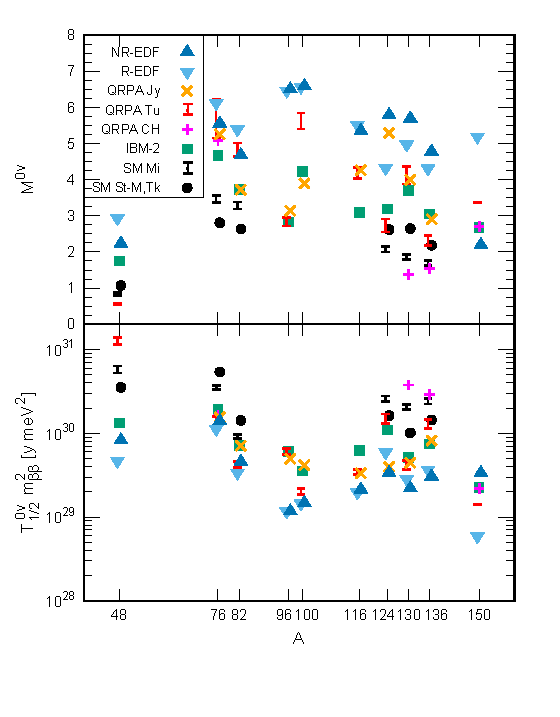
\includegraphics[width=0.8\linewidth]{Figures/NMEversusA.pdf}
    \caption[The various theoretically-determined nuclear matrix elements for selected \zeronubb~candidate isotopes.]
    {Top: The various theoretically-determined nuclear matrix elements for selected \zeronubb~candidate isotopes are shown.
    Bottom: The various models are in strong tension with one another and result in a large theoretical uncertainty for the half-life. Figure from \cite{Engel:NME}.}
    \label{fig:NME}
\end{figure}
Taking a model of light neutrino exchange, shown in \autoref{fig:0nuBB}, then $|f(m_i, U_{ei})|$ can be rewritten as
\begin{align}
        f(m_i, U_{ei})_{\textrm{light}} &= \frac{\langle m_{\beta\beta}\rangle}{m_e}
\end{align}
where $m_{\beta\beta}$ is the effective neutrino mass with
\begin{align}
    m_{\beta\beta}&=|\sum_iU^2_{ei}m_{\nu i}|.
    \label{eq:mbetabeta}
\end{align}
As the physical parameter $m_{\beta\beta}$ is isotope-independent, this becomes the figure-of-merit for comparing the results from experiments measuring the half-life of \zeronubb~decay from different isotopes. However, a large uncertainty is introduced due to the uncertainty in the nuclear matrix elements for each isotope.
In addition, possible values of $m_{\beta\beta}$ depend on the type of universe we are in, as shown in \autoref{fig:cuore-mbetabeta}.
If the masses of the neutrino obey inverted hierarchy, then the allowed values of $m_{\beta\beta}$ are within reach of current experiments with next-generation experiments being able to confidently rule out \zeronubb. However, for normal hierarchy, allowed values of $m_{\beta\beta}$ may be much lower. 
Due to the mono-energetic nature of \zeronubb, the sensitivity of an experiment can be determined from a few experimental parameters.
Each experiment can be reduced to a counting experiment in a window given by the energy resolution, $\Delta E$ of the experiment at the Q-value of \zeronubb.
For an experiment such as CUORE, with the source of \zeronubb~also the detectors, the number of signal events, $S$, in some time, $t$, would be given by
\begin{align}
    S &= \ln(2)\frac{\epsilon\cdot N \cdot t}{T^{0\nu}_{1/2}}
    \label{eq:signal_betabeta}
\end{align}
where $\epsilon$ is the signal detection efficiency and $N$ is the number of nuclei able to undergo \zeronubb.
Similarly, for the number of background events, $B$, in the same interval is given by
\begin{align}
    B &= b\cdot M \cdot t \cdot \Delta E
    \label{eq:background_betabeta}
\end{align}
where $b$ is the background rate per unit energy per unit detector mass and $M$ is the total active mass of the detector.
If $\Delta E$ is sufficiently small that the irreducible background from \twonubb~decays does not appreciably factor into the background and the background is therefore externally sourced and obeys Gaussian statistics, a $1\sigma$ half-life sensitivity is then given by
\begin{align}
    T^{0\nu}_{1/2}=\ln(2)\frac{\epsilon \cdot a_I \cdot N_A \cdot \eta}{W} \sqrt{\frac{M\cdot t}{b\cdot \Delta E}},
    \label{eq:sensitivity_long}
\end{align}
with $\eta$ as the number of nuclei of interest per molecule of the detector, e.g. 1 for CUORE's \teotwo~crystals, and where the number of candidate nuclei from \autoref{eq:signal_betabeta} is rewritten as
\begin{align}
    N &=M\frac{a_I \cdot N_A\cdot \eta}{W}
\end{align}
taking into account isotopic abundance, $a_I$, of the decaying isotope and its molar mass, $W$ along with Avogadro's number, $N_A$.
For an experiment that searches for \zeronubb, maximizing this sensitivity is of paramount importance, and the most experimentally-relevant factors result in a common rewriting of the sensitivity as
\begin{align}
S &\propto a_I \sqrt{\frac{M \cdot t}{b \cdot \Delta E}}.
\label{eq:sensitivity_short}
\end{align}
This means that an experiment searching for \zeronubb~gains by increasing the isotopic abundance of the decay of interest, increasing its live-time, $M\cdot t$, decreasing its background, and improving its energy resolution.
Many experiments enrich their isotope of choice in order to increase their sensitivity, while CUORE benefits from the relatively high natural abundance of \teonethirty, shown in \autoref{fig:q_vs_ia-color}, and does not need to undergo the expense process of isotope enrichment.
A high Q-value also helps to decrease the background as \gamma~backgrounds generally decrease at higher energies and it is equally important to avoid other \gamma~peaks from decays near the Q-value.
For example, in CUORE, two \gamma~particles emitted from $^{60}\textrm{Co}$ decays may be absorbed simultaneously in a detector with an energy of approximately 2605 keV.
Since this is close the to the Q-value of 2528 keV for \teonethirty, this requires $\Delta E$ small enough to distinguish these background events from the possible signal.
CUORE's design goal of 5 keV resolution is more than enough to accomplish this.
In practice, experiments such as CUORE with a precise energy resolution suffer from having a segmented detector, as the materials used to hold the detectors in place also contribute to the background.
Other experiments such as those that search for \zeronubb~decay in $^{136}$Xe are able to scale up their mass much easier as it is all one continuous volume, but suffer from having significantly less precise energy resolution.
A further discussion of other experiments in the field is in \autoref{sec:State of Neutrinoless Double Beta Decay Experiments}.
\begin{figure}[htbp]
    \centering
    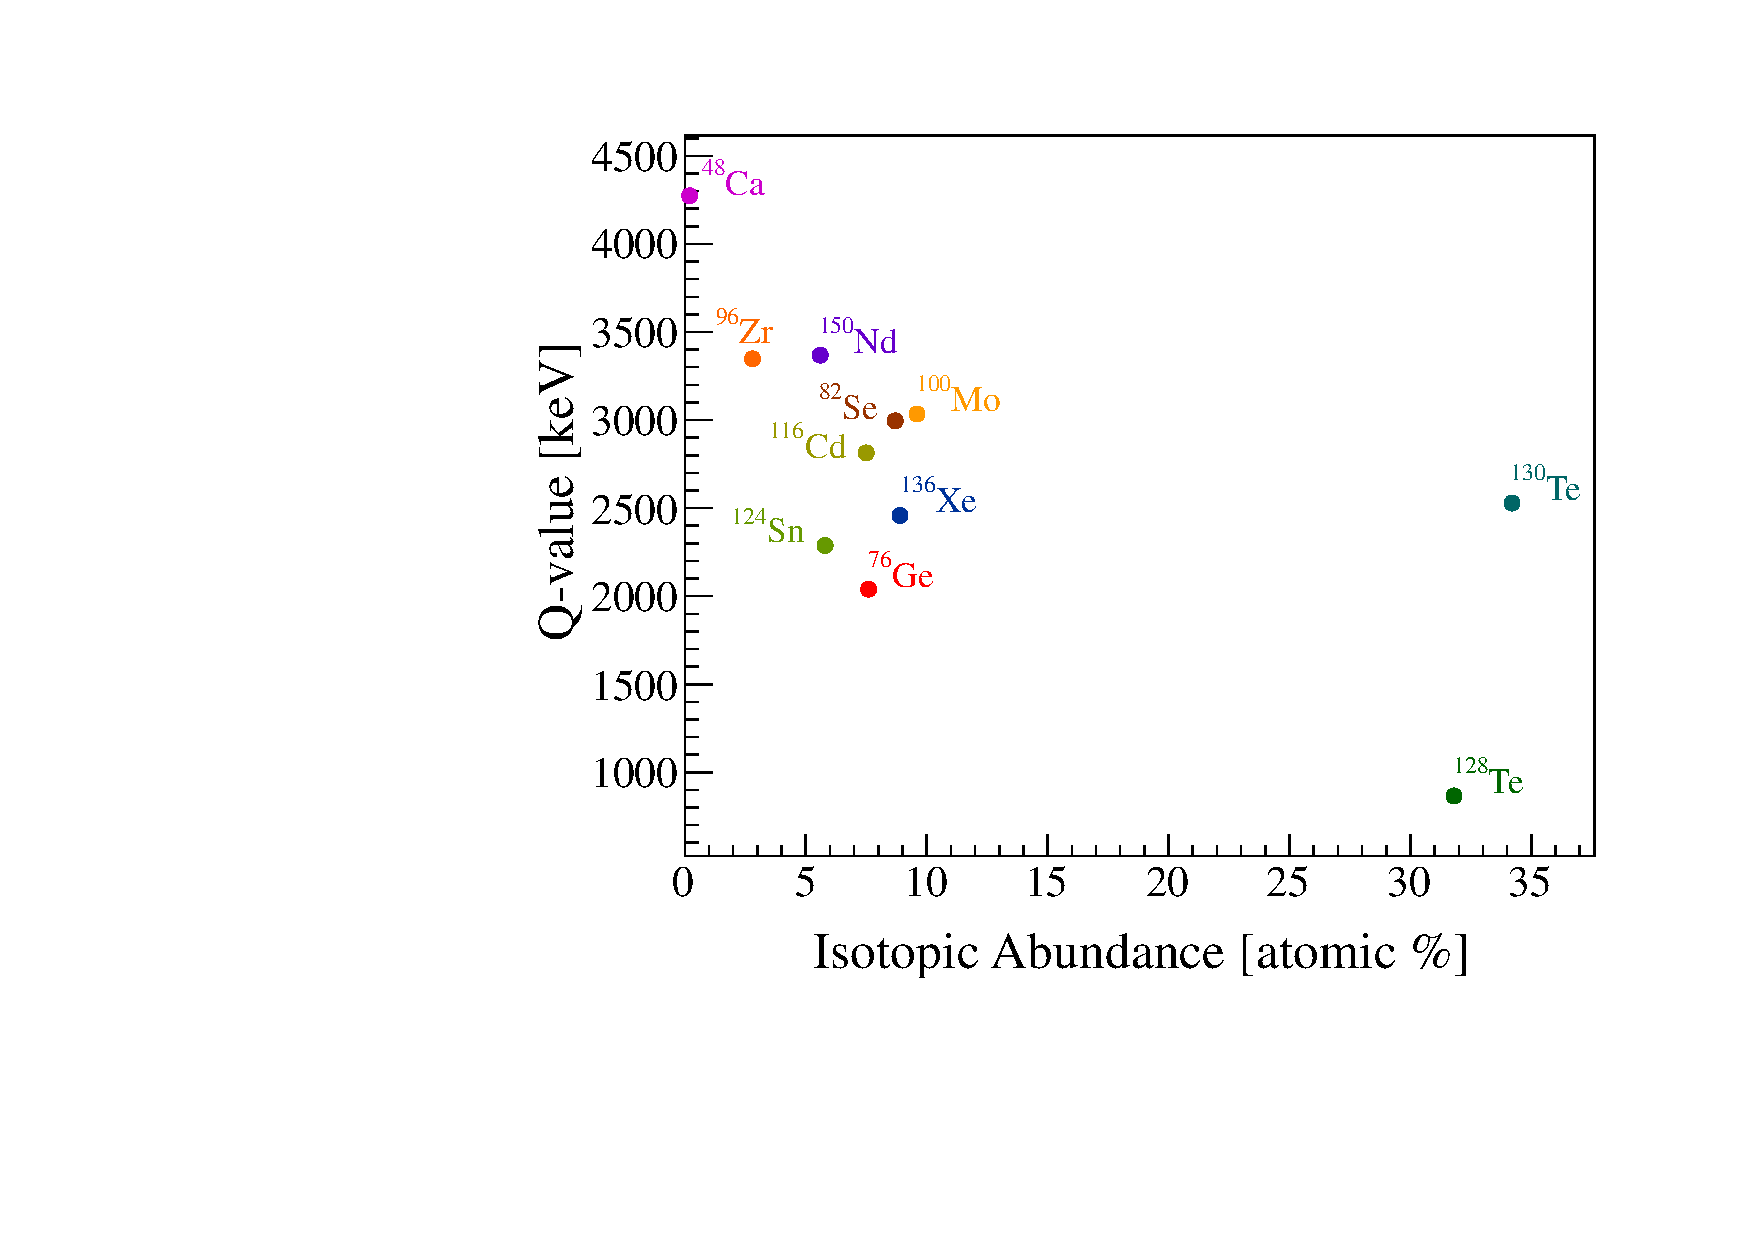
\includegraphics[width=0.7\linewidth]{Figures/q_vs_ia-color.pdf}
    \caption[The isotopic abundances and q-values of \zeronubb~candidate nuclei.]
    {The isotopic abundances and q-values of \zeronubb~candidate nuclei.
    Note that the \teonethirty~isotopic abundance is significantly higher for natural tellurium than for other elements.}
    \label{fig:q_vs_ia-color}
\end{figure}
A goal of many next-generation \zeronubb~decay experiments is to have a negligibly small background near the Q-value.
This changes the calculation in \autoref{eq:sensitivity_short} to be merely
\begin{align}
    S &\propto a_I \cdot M \cdot t
\end{align}
which is a significant increase in sensitivity, especially as experiments work to scale up in mass to become more sensitive to longer half-lives.
\subsection{Neutrinoless Double-Beta Decay with Majoron Emission}
\label{ssec:Neutrinoless Double-Beta Decay with Majoron Emisison}
\zeronubb~decays as shown in \autoref{eq:doubleneutrondecay} and \autoref{eq:doubleprotondecay} where only electrons are emitted are not the only possible decay mode for these candidate nuclei.
Some proposed models of \zeronubb~decay predict the existence of another particle, called a majoron, that is emitted during the decay.
In the original theory, these majorons are the Goldstone boson that is created during a spontaneous global breaking of B-L symmetry \cite{CHIKASHIGE1981265}.
The Majorons in the original models were posited as belonging to either a singlet, doublet, or triplet state, but the doublet and triplet states have been ruled out by precision measurements of the Z boson width at the LEP experiment \cite{ALEPH:2005ab}.
However, a whole class of models have now been developed that predict similar phenomena as the original theories where either one or two light, neutral bosons\footnote{Although the original majoron was postulated as a Goldstone boson, the majoron in these models may or may not be a Goldstone boson.}
are emitted during a neutrinoless double-beta decay \cite{HIRSCH19968}.
Decays emitting a single majoron are denoted as \zeronubbonechi, and decays emitting two majorons are denoted as \zeronubbtwochi.
These models are classified into two types (I and II) where either lepton number is (type I) violated in neutrinoless double-beta decay, i.e. the lepton number of the majoron is zero, or where lepton number is not (type II) violated, i.e. the lepton number of the majoron cancels out the $L=\pm2$ from the emitted electrons.
In models of type II, \zeronubb~decay without majoron emission is forbidden, whereas for models of type I, \zeronubb~decay is allowed.
However, as \zeronubb~decay has yet to be observed in the laboratory, these two types of models are indistinguishable from one another.
The types of models for majoron decay are summarized in \autoref{tab:Majoron Decay Modes}. 
\begin{table}[H]
    \centering
\begin{tabular}{lllcc}
\hline \hline
Model   & Decay Mode & Goldstone Boson & Lepton Number & Spectral Index \\ \hline
IB      & \zeronubbonechi & no              & 0    & 1              \\ 
IC      & \zeronubbonechi & yes             & 0    & 1              \\ 
ID      & \zeronubbtwochi & no              & 0    & 3              \\ 
IE      & \zeronubbtwochi & yes             & 0    & 3              \\ 
\hline
IIB     & \zeronubbonechi & no              & -2   & 1              \\ 
IIC     & \zeronubbonechi & yes             & -2   & 3              \\ 
IID     & \zeronubbtwochi & no              & -1   & 3              \\ 
IIE     & \zeronubbtwochi & no              & -1   & 7              \\ 
IIF     & \zeronubbonechi & no              & -2   & 3              \\ 
\hline
``bulk" \cite{Mohapatra:2000px} & \zeronubbonechi & no              & 0    & 2              \\
\hline \hline
\end{tabular}
\caption[The majoron models and their associated decay modes.]
{The majoron models and their associated decay modes.
Also shown is if the majoron is a Goldstone boson, the associated lepton number of the majoron, and the spectral index of the decay.
In models of type II \zeronubbtwochi, each majoron has an associated lepton number which precisely cancels out the $\Delta L$ carried by the electrons in these \zeronubbtwochi~decays.}
\label{tab:Majoron Decay Modes}
\end{table}
Experimentally, the energy spectrum of the two electrons emitted varies by the spectral index of each of the models according to
\begin{align}
    S(E_{\textrm{sum}}) &= \int_1^{E_{sum}-1}F(Z, E_1) E_1 p_1 F(Z, E_2) E_2 p_2 (E_{tot}-E_1-E_2)^n dE_1 dE_2 \delta(E_{sum}-E_1-E_2)
    \label{eq:spectral index}
\end{align}
where $E_{\textrm{sum}}$ is the summed energy of the electrons, $F(Z, E)$ is the Fermi function for the daughter nucleus with atomic number Z, $E_i$ and $p_i$ are the energy and momentum of each particle, respectively, and $n$ is the spectral index.
The Fermi function comes from a correction due to Coulomb interactions between the emitted electrons and the daughter nucleus in the decay.
To lowest order, this function is given by 
\begin{align}
    F(Z,E) &= 4(2 p \rho)^{2(\gamma - 1)}e^{y\pi} \frac{|\Gamma(\gamma+iy)|^2}{|\Gamma(2\gamma+1)|^2}\frac{1+\gamma}{2} \\
    \gamma &= (1-(\alpha Z)^2)^{1/2} \\
    y &= \alpha Z W / p
\end{align}
where $\rho$ is the nuclear radius, $p$ is the momentum of the electron, and $\Gamma(x)$ is the gamma function\footnote{$\Gamma(z)=\int_0^\infty x^{z-1}e^{-x}dx$} \cite{PhysRev.150.846}.
The spectrum for \twonubb~decay corresponds to a spectral index of 5.
The energy spectrum for each spectral index of \zeronubb~with majoron emission is shown in \autoref{fig:Majoron Spectrum}.

\begin{figure}[htbp]
    \centering
    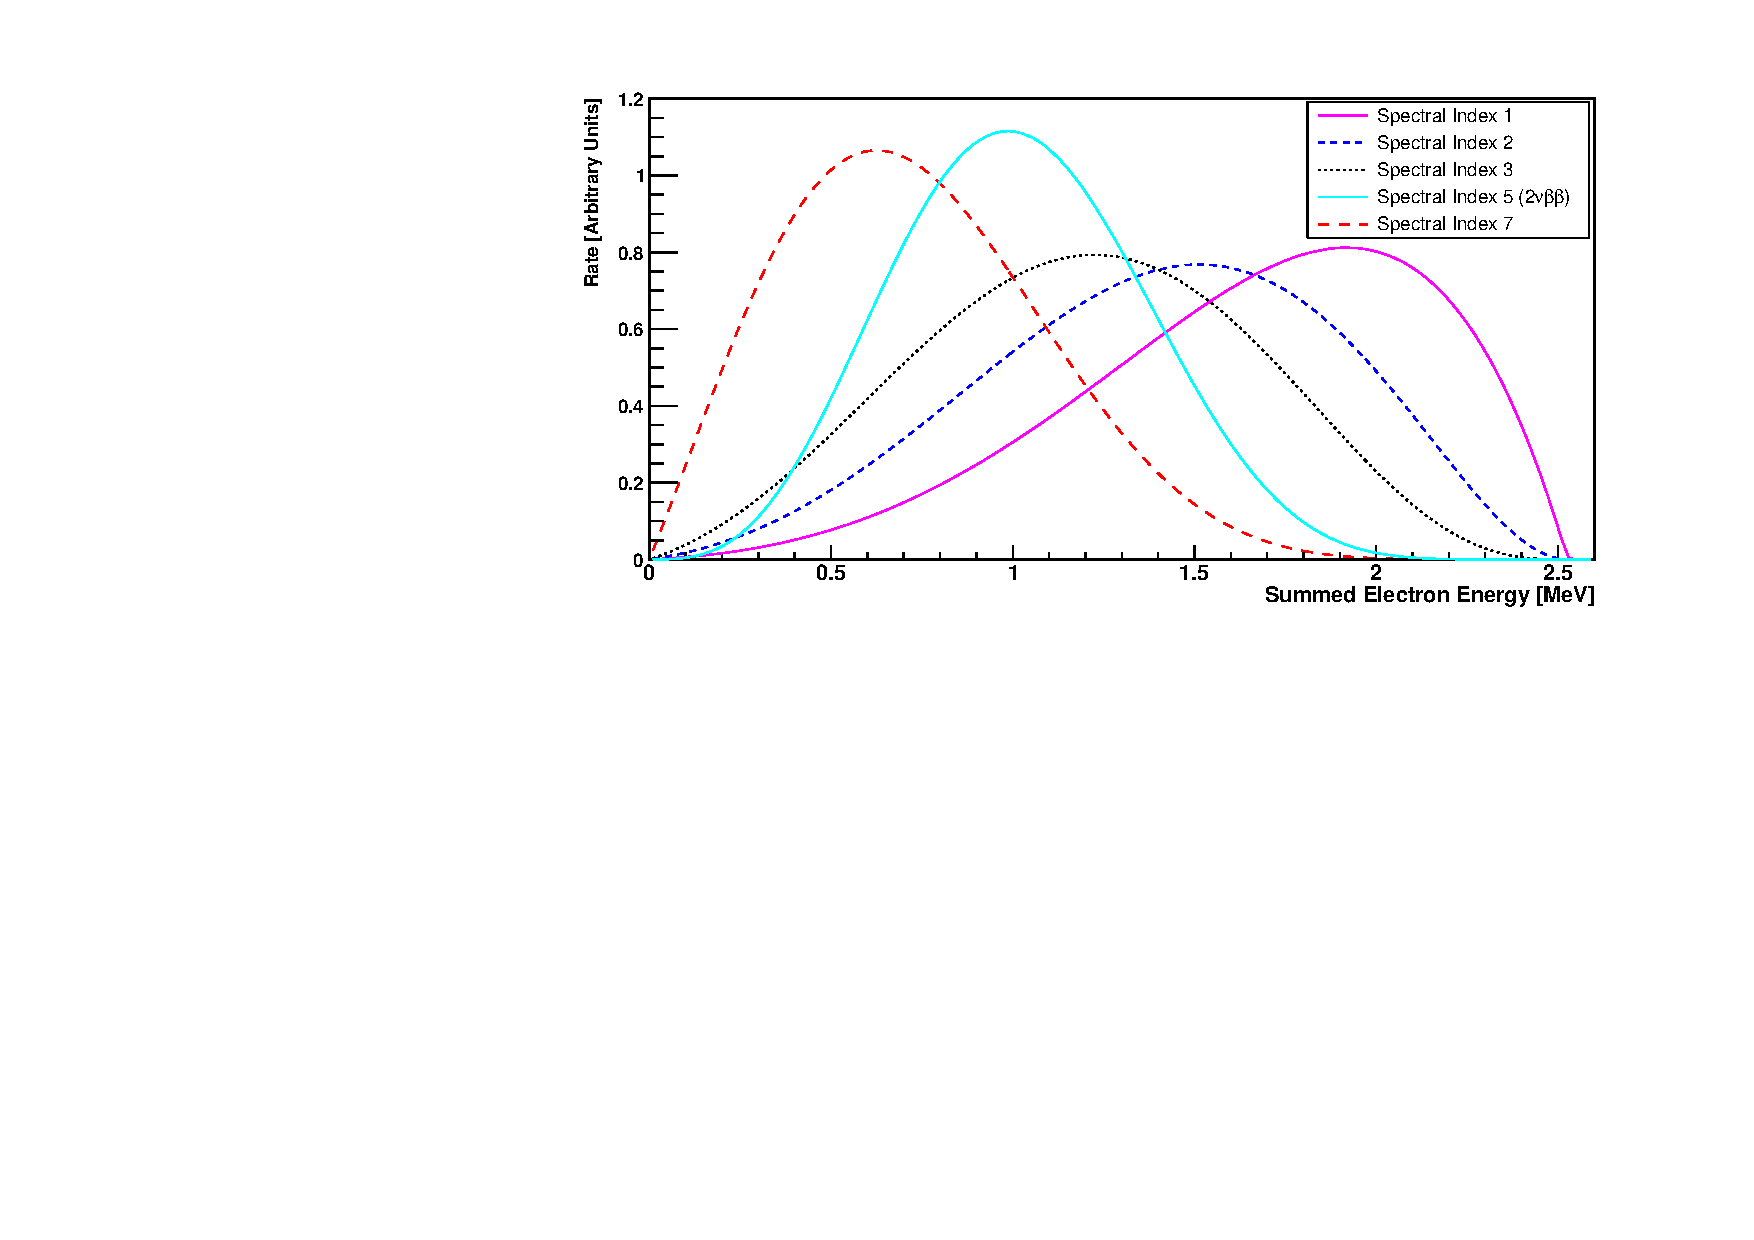
\includegraphics[width=0.9\linewidth]{Figures/EnergySpectrum_fixedFermi.pdf}
    \caption[The summed electron energy spectra for multiple types of Majoron emission according to spectral indices 1, 2, 3, 5, and 7.]
    {The summed electron energy spectra for multiple types of Majoron emission according to spectral indices 1, 2, 3, 5, and 7.
    Spectral index 5 corresponds to \twonubb~and is not a Majoron decay, but is shown for context.
    The integrals of each of the spectra are normalized to 1.}
    \label{fig:Majoron Spectrum}
\end{figure}

\section{State of Neutrinoless Double-Beta Decay Experiments}
\label{sec:State of Neutrinoless Double Beta Decay Experiments}
In addition to CUORE, many other experiments are currently searching and have searched for \zeronubb~ decay. Some of these experiments are listed below and the current status of the field is shown in \autoref{fig:cuore-mbetabeta}.
As noted before in \autoref{sec:Double Beta Decay} and \autoref{sec:Neutrinoless Double Beta Decay}, the signatures of \zeronubb~ and \twonubb~ decays are a nucleus that interchanges two neutrons and two protons, along with the emission of two electrons and, in the case of \twonubb~decay or Majoron emission, two neutrinos and up to two Majorons.
Since the half-lives of these decays are so large, (consider that the Universe is only $1.38\times10^{9}~\textrm{yr}$ old) an experiment needs to have extremely low background levels in order to be able to even observe these events.
As an example, a 1-tonne experiment searching for \zeronubb~decay would expect only $\mathcal{O}(10)$ events per year.
This is generally realized in experiments by going to deep underground laboratories to escape cosmic radiation sources and by having pure and clean materials in and near the detector and sources.
Also, due to the energies being produced according to a spectrum, all of the backgrounds with energy up to the Q-value will reduce the sensitivity of the measurement.
The experiments listed here all seek to identify these signals using a particular technology or set of technologies, some of which, especially in the case of GERDA and MAJORANA, are quite similar to CUORE's.
Despite the wide array of technologies, all the experiments below, including CUORE, seek to identify these decays by honing in on and measuring the emitted electron energies as the summed energy spectrum is well-defined as a sharp peak for \zeronubb~or as a broader spectrum for \twonubb~for Majoron emission.

\begin{figure}[htbp]
\centering
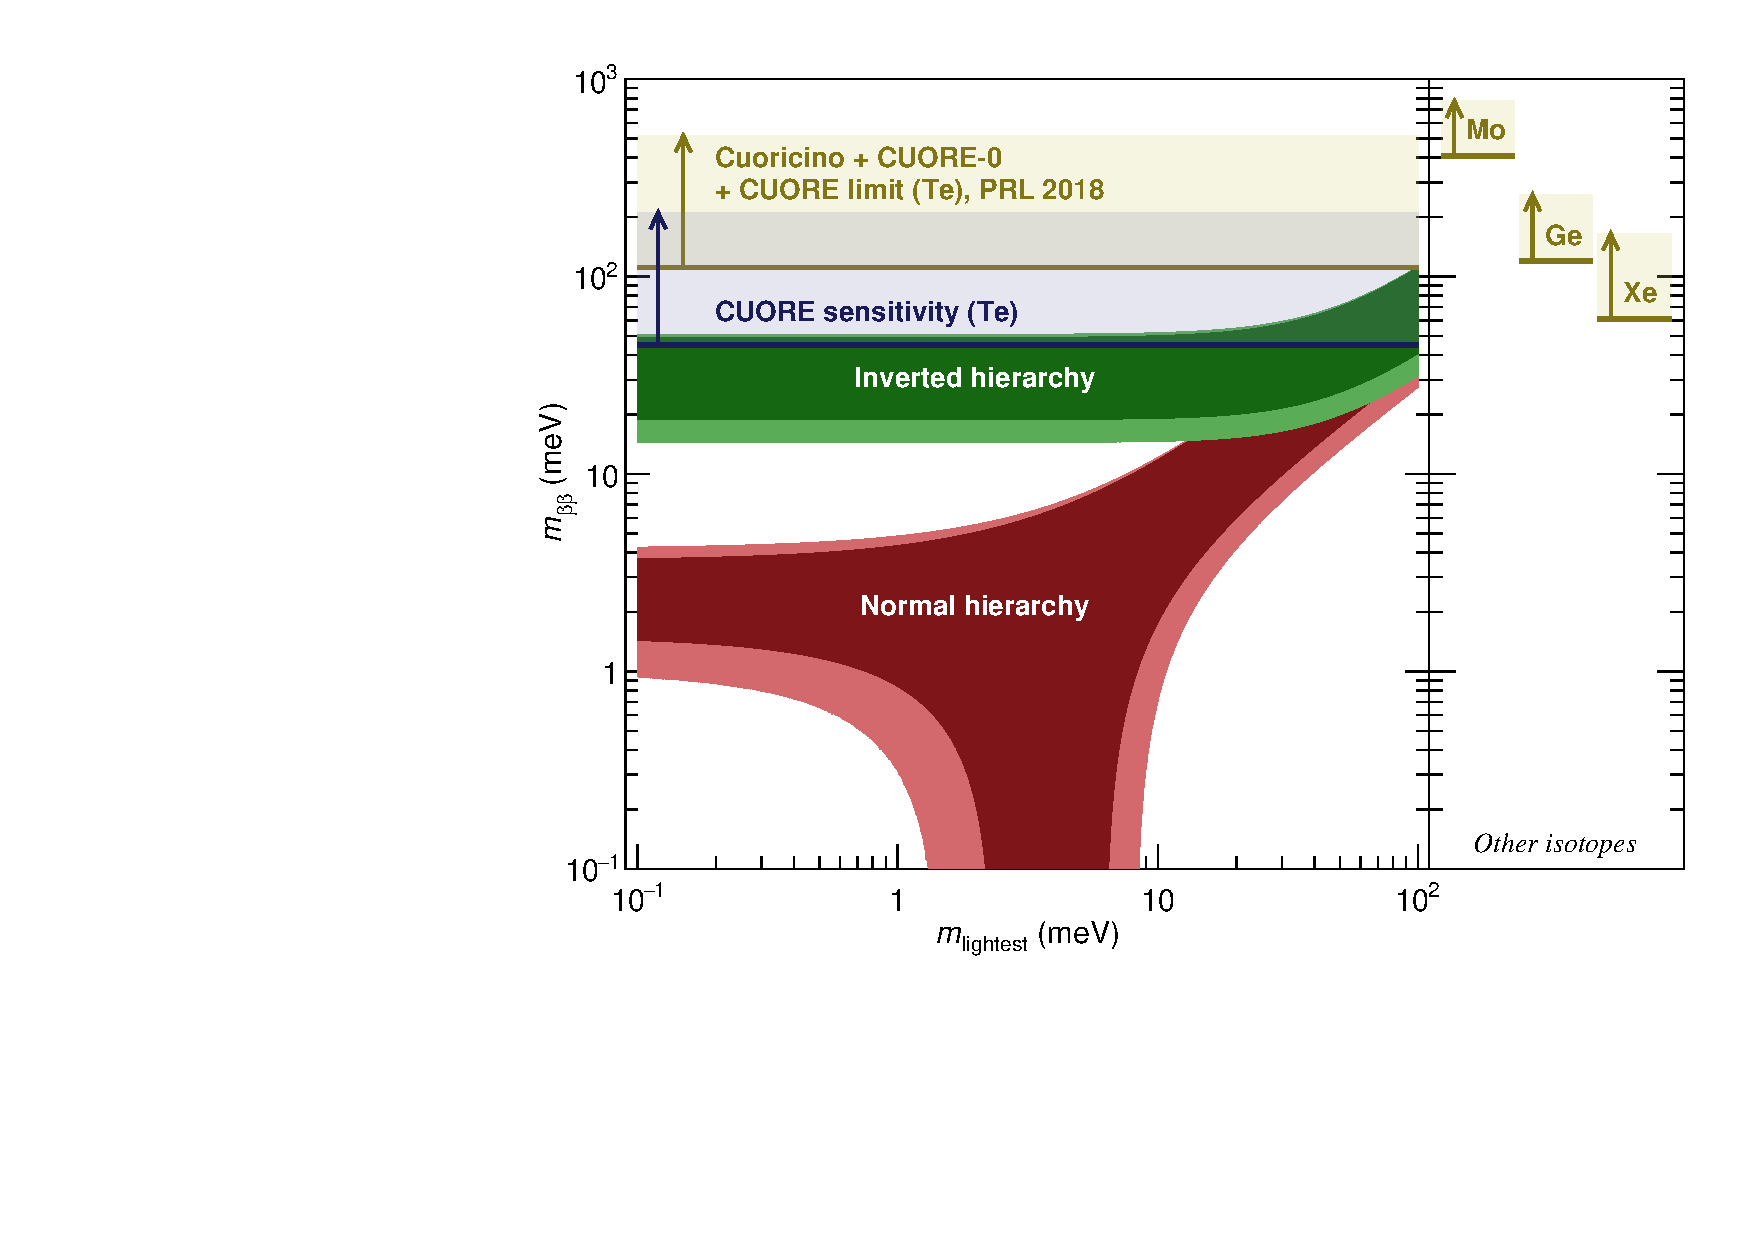
\includegraphics[width=0.7\linewidth]{Figures/M_bb_vs_mlightest_CL_2018.pdf}
\caption[The current status of the field of \zeronubb.]
{The current status of the field of \zeronubb. See \autoref{eq:mbetabeta} for the definition of $m_{\beta\beta}$ and $m_{\textrm{lightest}}$ corresponds to the mass of the lightest neutrino in either normal or inverted hierarchy.
The previous experiments in the line of CUORE, CUORE-0 and Cuoricino, have their combined $^{130}$Te result and the results for Mo, Ge, and Xe are shown from NEMO-3, GERDA, and KamLAND-Zen, respectively.}
\label{fig:cuore-mbetabeta}
\end{figure}

\subsection{GERDA}

The GERmanium Detector Array (GERDA) Experiment is currently searching for \zeronubb~at the Laboratori Nationali del Gran Sasso (LNGS) using  $^{76}$Ge as the source \cite{Agostini:2017iyd}.
Unlike in CUORE, the source is enriched from the natural $7.8\%$ abundance up to $86\%$ and acts acts both the source and the detector of \zeronubb.
In the most recent phase of GERDA, Phase II, 37 enriched detectors, 35.6 kg, are assembled along 6 strings around a central string with 3 unenriched detectors.
These detectors are then submerged in a 64 $\textrm{m}^3$ LAr cryostat inside a 590 $\textrm{m}^3$ water tank.
The water acts as a passive shield for the experiment, while the LAr also acts as an active shield.
One of the advantages that CUORE shares with GERDA over other detector technologies is the excellent energy resolution which, recalling \autoref{eq:sensitivity_short} inversely effects the sensitivity.
GERDA also takes advantage of the pulse-shape discrimination (PSD) between \zeronubb-like events and $\gamma$-like events in 30 broad energy (BEGe) detectors in addition to scintillation light from the surrounding LAr.
With this, the background at $Q_{\beta\beta}$ for the BEGe detectors is low enough at $(0.07^{+1.1}_{-0.5})\times 10^{-3} ~\textrm{counts} \cdot  (\textrm{keV} \cdot \textrm{kg} \cdot \textrm{yr})^{-1}$ allowing for the experiment to be considered background-free at the design exposure of $100 \textrm{kg \cdot yr}$.
A diagram of the GERDA experimental setup is shown in \autoref{fig:gerda-labelled}.
\begin{figure}[tbph]
\centering
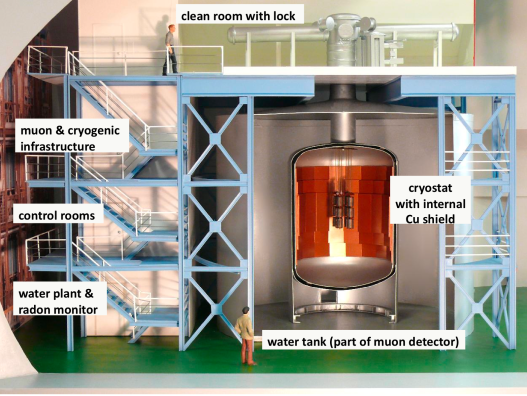
\includegraphics[width=0.7\linewidth]{Figures/gerda-view.png}
\caption[Diagram of the GERDA detector.]
{Diagram of the GERDA detector.
Liquid argon is also inside the copper shielding with the detectors submerged.}
\label{fig:gerda-labelled}
\end{figure}

\subsection{MAJORANA}
The \textsc{Majorana Demonstrator}, shown in \autoref{fig:MajoranaDemonstrator} is another experiment using $^{76}$Ge to search for \zeronubb~located in the Sanford Underground Research Facility in South Dakota.
This experiment deploys 30 kg of Ge enriched to 87\% $^{76}$Ge and 14 kg of Ge with natural 7.8\% $^{76}$Ge \cite{1742-6596-606-1-012004}.
The detection principles for the \textsc{Demonstrator} are similar to that of GERDA, but there are differences in detector operation and construction, particularly as the \textsc{Demonstrator} does not have the active lAr veto from GERDA, but has a more stringent materials selection and parts processing which results in their background rate of $1.6^{+1.2}_{-1.0}\times10^{-3} ~\textrm{counts}\cdot(\textrm{keV}\cdot \textrm{kg} \cdot \textrm{yr})^{-1}$.
\begin{figure}
    \centering
    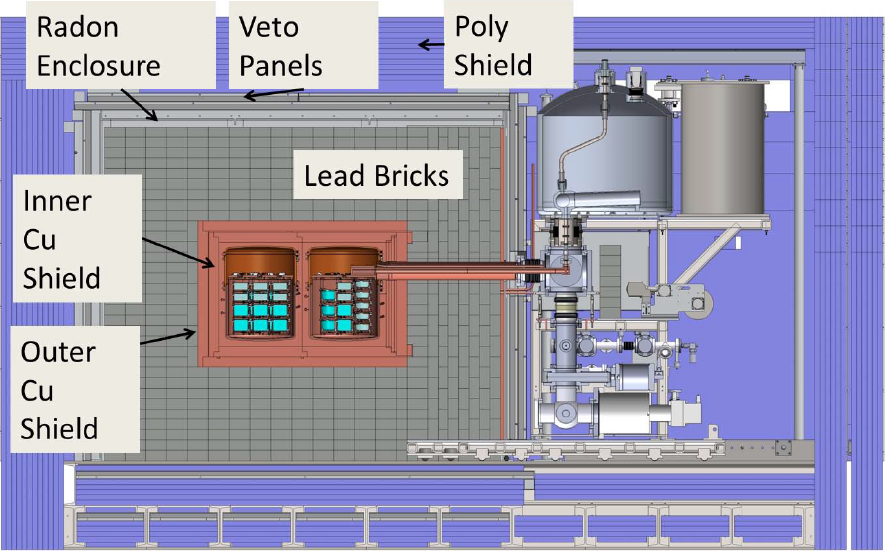
\includegraphics[width=0.8\linewidth]{Figures/MajoranaDemonstrator.png}
    \caption[The \textsc{Majorana Demonstrator} experimental apparatus.]
    {The \textsc{Majorana Demonstrator} experimental apparatus.
    The external active and passive shielding is shown enclosing the detectors inside the two cryostats.
    Figure from \cite{1742-6596-606-1-012004}.}
    \label{fig:MajoranaDemonstrator}
\end{figure}
\subsection{KamLAND-Zen}
The Kamioka Liquid Scintillator Antineutrino Detector Zero-neutrino double-beta decay search (KamLAND-Zen) searches for \zeronubb~in 90.8\% enriched $^{136}$Xe \cite{KamLAND-Zen:2016pfg}.
This experiment uses the existing infrastructure from the KamLAND experiment, with a balloon filled with enriched Xe in the center of the KamLAND liquid scintillator.
The detector uses the Xe-doped (2.9\% by weight) liquid scintillator acting as both the source and detector of \zeronubb.
Xe benefits from self-shielding due to the attenuation length of gammas in xenon which allows for reduced levels of background in the innermost volume.
This is a distinct advantage over experiments such as CUORE, MAJORANA, and GERDA, as their detectors need to be held in place and cannot self-shield as a result.
Also, the detector mass is relatively easily scalable by the size of the balloon and does not require a full reconstruction of the surrounding veto from the KamLAND experiment.
In addition, by taking out the Xe or depleting the Xe in the liquid scintillator, the experiment can make an on/off measurement to confirm any possible measurement of \zeronubb. 
However, the energy resolution of the KamLAND-Zen is significantly worse than the $\mathcal{O}(\textrm{keV})$ resolution in these experiments which introduces the tail of the \twonubb spectrum as an irreducible background.
A diagram of the KamLAND-Zen detector is shown in \autoref{fig:kamlandzen}.
\begin{figure}[tbph]
\centering
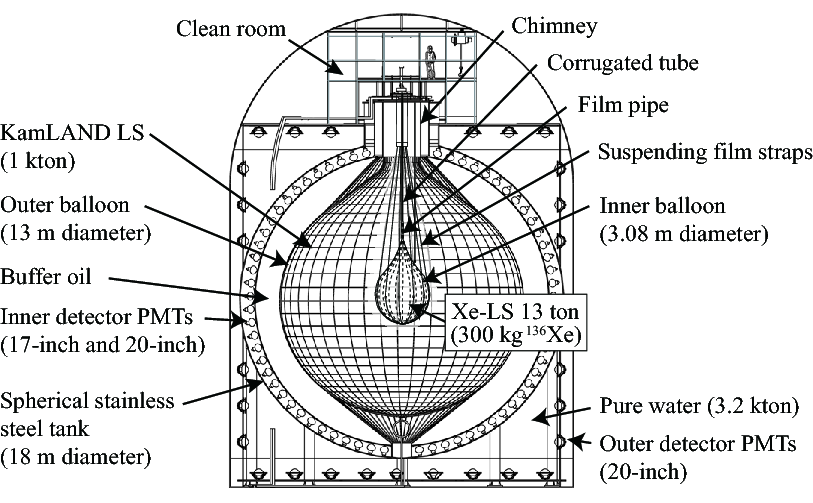
\includegraphics[width=0.7\linewidth]{Figures/KamlandZen}
\caption[A schematic of the Kamland-Zen experimental apparatus.]
{A schematic of the Kamland-Zen experimental apparatus.
The Xe-loaded liquid scintillator is held within the balloon at the center.
Figure from \cite{::2015uaa}.}
\label{fig:kamlandzen}
\end{figure}

\subsection{EXO-200}
The Enriched Xenon Observatory (EXO-200) searches for \zeronubb~ with 200 kg of Xe with 80.6\% enriched $^{136}$ Xe in a liquid xenon time projection chamber (TPC) and is located in the Waste Isolation Pilot Plant near Calsbad New Mexico \cite{Albert:2017owj}.
The TPC collects both charge and light signals from energy depositions in the Xe and reconstructs them as either single-site or multi-site events.
This provides discrimination between the multi-site \gamma~backgrounds and the single-site signal.
\begin{figure}[htbp]
    \centering
    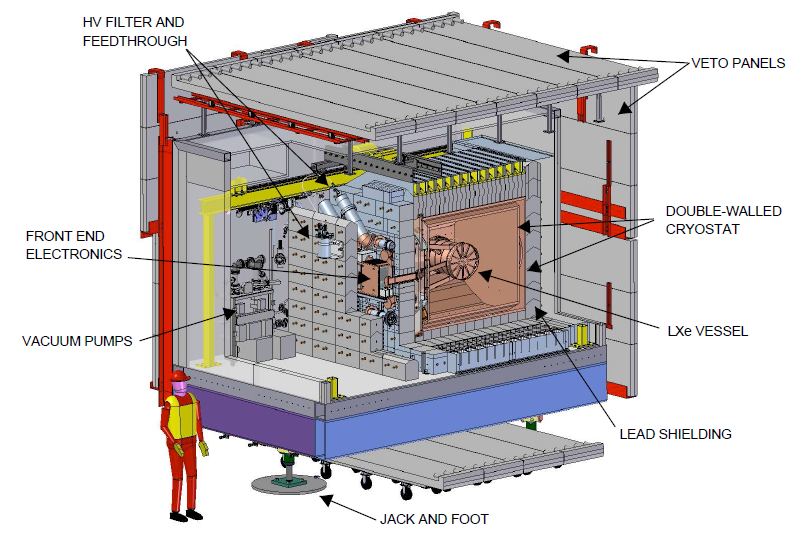
\includegraphics[width=0.7\linewidth]{Figures/EXO.png}
    \caption[The EXO-200 detector setup.]
    {The EXO-200 detector setup.
    The LXe TPC is contained within the cryostat, with the entire setup surrounded by a muon veto.
    Figure from \cite{Auger:2012gs}.}
    \label{fig:EXO}
\end{figure}

\subsection{NEMO-3}
The Neutrino Ettore Majorana Observatory (NEMO-3) collected \twonubb~data from multiple isotopes including $^{100}$Mo, $^{82}$Se, $^{130}$Te, $^{116}$Cd, $^{150}$Nd, $^{96}$Zr, and $^{48}$Ca \cite{Bongrand:2011ei}.
NEMO-3 also searched for \zeronubb~in $^{100}$Mo, $^{82}$Se, $^{48}$Ca, and $^{150}$Nd \cite{Bongrand:2011ei}\cite{Arnold:2016qyg}\cite{Arnold:2016ezh}.
Unlike the other experiments listed in this section, NEMO-3 did not utilize a ``detector = source" method, instead using separate detectors and sources.
An advantage of this method is that the two emitted electrons can be tracked and measured separately, which is a clear signal that a decay occured as a vertex can be reconstructed along with the energies of the particles.
An example track in NEMO-3 is shown in \autoref{fig:nemo3393042373top2}.
Another advantage is that the source foil can be easily replaced with other isotopes while leaving the rest of the detector apparatus unchanged.
However, this is a constraint on the size of the source, as it needs to be small enough for electrons to traverse and be detected outside, yet, as shown in \autoref{eq:sensitivity_short}, the number of decays scales with the source mass.
\begin{figure}[htbp]
\centering
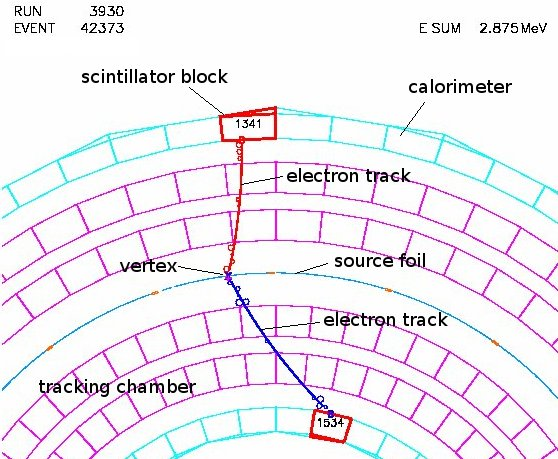
\includegraphics[width=0.7\linewidth]{Figures/nemo3_3930_42373_top_2}
\caption[An example double-beta decay candidate event from NEMO-3.]{An example double-beta decay candidate event from NEMO-3.
The electrons are emitted from a nucleus in the source foil and deposit energy in the calorimeter after leaving tracks in the tracking chamber.}
\label{fig:nemo3393042373top2}
\end{figure}
